% -----------------------------------------------
% chktex-file 44
\documentclass[../index.tex]{subfiles}
\begin{document}

% -------------------------------------

\renewcommand{\sectiontitle}{Organization of a basic compiler}
\section{\sectiontitle}

% ---------------------------
\renewcommand{\currenttitle}{Front-end and back-end}
\begin{frame}{\currenttitle}
  Much like a full-stack web application, we can split the compiler into a
  \textbf{front-end} and a \textbf{back-end}: \\[2em]

  \begin{tikzpicture}[%
    wrapper/.style={matrix of nodes, nodes=typetag, row sep=1em},
    container/.style={draw, inner sep=1ex},
    typetag/.style={draw=gray, inner sep=1ex, anchor=west},
    title/.style={draw=none, inner sep=0pt}
  ]
    \matrix[wrapper] (Frontend) {
      |[title]|Front-end \\
      Lexical analysis \\
      Parsing \\
      Semantic analysis \\
      Intermediate code generation \\
    };
    \matrix[wrapper, right=of Frontend.north east, matrix anchor=north west] (Backend) {
      |[title]|Back-end \\
      More optimization \\
      Code generation \\
    };

    \node[container, fit=(Frontend)] {};
    \node[container, fit=(Backend)] {};
  \end{tikzpicture}
\end{frame}

% ---------------------------
\begin{frame}{\currenttitle}
  \onslide<+->{
    The front-end:
    \begin{itemize}
      \item Deals with the details of the source language
      \item Verifies that the programmer's code is correct
      \item Generates an intermediate representation that the backend can handle
    \end{itemize}
  }

  \onslide<+->{
    The back-end:
    \begin{itemize}
      \item Is ignorant to the details of the source language
      \item Performs optimizations specific to the target machine
      \item Generates the final executable program
    \end{itemize}
  }
\end{frame}

% ---------------------------
\begin{frame}{\currenttitle}
  Different targets need different output code. For example:

  \begin{itemize}
    \item<2-> Different CPU architectures have different sets of instructions and quirks
      \begin{itemize}
        \item e.g. the x86 instruction set is different from ARM or MIPS sets
      \end{itemize}
    \item<3-> Web assembly bytecode is different from other bytecode, such as JVM bytecode
  \end{itemize}

  \vspace*{1em}
  \onslide<4->{Thus, we need different compilers for different targets}
\end{frame}

% ---------------------------
\begin{frame}{\currenttitle}
  \onslide<+->{What does the separation between front-end and back-end allow us
  to do?} \\[2em]

  \onslide<+->{With \textbf{\texttt{M}} front-ends for \textbf{\texttt{M}}
  source languages\ldots{}}
  \onslide<+->{and \textbf{\texttt{N}} back-ends for \textbf{\texttt{N}}
    target machines,} \\[1em]
    
  \hspace*{2em}
  \onslide<+->{\textit{we can write \textbf{\texttt{M x N}} compilers}}

\end{frame}

% ---------------------------
\begin{frame}{\currenttitle}
  Often, it may be even more meaningful to distinguish between three sections:

  \begin{itemize}
    \item<+-> Front-end concerned with parsing and language-specific analysis
      and optimization
    \item<+-> Intermediate phases that analyze and optimize a language-agnostic
      IR
    \item<+-> Back-end code generation concerned with the details of the target
      machine
  \end{itemize}
\end{frame}

% -------------------------------------

\renewcommand{\sectiontitle}{Syntax analysis}
\section{\sectiontitle}

% ---------------------------
\renewcommand{\currenttitle}{Understanding the source code}
\begin{frame}{\currenttitle}
  \vspace*{1em}
  We want to parse source code into data that we can analyze and transform. \\[1.5em]

  Typically, compilers first construct an \textbf{abstract syntax tree (AST)}:

  \begin{center}
    \begin{tikzpicture}[
      font=\ttfamily,
      nodes={draw=none},
      level distance=0.8cm,
      ->
    ]
      \node (Code) at (0,-1.5) [inner sep=0.5em, outer sep=2] {
          a = b + c * d("hello");
      };

      \node (AST) at (4,0) {=}
        child {node {a}}
        child {node {+}
          child {node {b}}
          child {node {*}
            child {node {c}}
            child {node {call}
              child {node {d}}
              child {node {"hello"}}
            }
          }
        }
      ;
    \end{tikzpicture}
  \end{center}
\end{frame}

% ---------------------------
\begin{frame}{\currenttitle}
  \onslide<+->{
    It's the job of the \textbf{parser} to convert the \textbf{tokens}
    \texttt{a}, \texttt{=}, \texttt{b}, \texttt{+}, \ldots{} into the syntax
    tree \\[1em]
  }

  \onslide<+->{
    But before that, how do we get those tokens?
  }
\end{frame}

% ---------------------------
\renewcommand{\currenttitle}{Lexical analysis}
\begin{frame}[fragile]{\currenttitle}
  To convert textual source code into \textbf{tokens}, we must perform
  \textbf{lexical analysis}: \\[1em]

  Given the source code: 

  \newcommand{\token}[2]{%
    {
      \scriptsize
      \begin{tabular}{|l |l |}
        \hline
        \textbf{#2} & #1 \\
        \hline
      \end{tabular}
    }
  }

  \begin{lstlisting}[language=C++,xleftmargin=1.5em]
int main() {
  return 1;
}
  \end{lstlisting}

  The \textbf{lexer / lexical analyzer} might spit out the tokens: \\[0.5em]

  \begin{tikzpicture}
    \newcommand{\tokennode}[2]{
      \node [shape=rectangle, anchor=west, outer sep=.0] {
        \token{#1}{#2}
      };
    }

    \matrix[ampersand replacement=\&, matrix of nodes, align=left] {
      \tokennode{int}{Type}   \& \tokennode{main}{Identifier} \& \tokennode{(}{Symbol}        \\
      \tokennode{)}{Symbol}   \& \tokennode{\{}{Symbol}       \& \tokennode{return}{Keyword}  \\
      \tokennode{1}{Literal}  \& \tokennode{;}{Symbol}        \& \tokennode{\}}{Symbol}       \\
    };
  \end{tikzpicture}
\end{frame}

% ---------------------------
\begin{frame}[fragile]{\currenttitle}
  To implement a lexer, we can:

  \begin{itemize}
    \item Manually scan and lookahead the input characters
    \item Implement a \textbf{finite state machine}
  \end{itemize}

  In practice, the latter method typically uses a \textbf{lexer generator} to
  generate the state machine based on rules
\end{frame}


% ---------------------------
\begin{frame}[fragile]{\currenttitle}
  \only<+>{
    To give an idea, a finite state machine to recognize a floating-point:
  }

  \vspace*{1em}

  \newcommand{\statenode}[2]{\node [state] (#1) [#2] {$#1$}}
  \begin{center}
    \begin{tikzpicture}[shorten >= 1pt, node distance=2cm, on grid, auto, font=\ttfamily]
      \tikzstyle{every state}=[fill={rgb:black,1;white,10}]

      \node [state, initial]    (s_0)                       {$s_0$};
      \node [state]             (s_1) [above right of=s_0]  {$s_1$};
      \node [state, accepting]  (s_2) [below right of=s_1]  {$s_2$};
      \node [state, accepting]  (s_3) [right of=s_2]        {$s_3$};

      \path[->]
        (s_0) edge                node {+/-} (s_1)
              edge                node {0-9} (s_2)
        (s_1) edge                node {0-9} (s_2)
        (s_2) edge  [loop below]  node {0-9} ()
              edge                node {.}   (s_3)
        (s_3) edge  [loop below]  node {0-9} ()
        ;
    \end{tikzpicture}
  \end{center}

  \only<+>{
    \begin{itemize}
      \item Start on $s_0$
      \item Read input and move accordingly until the end of the input
        \begin{itemize}
          \item If we end on a double-ringed (accepting) state, the input
            string is a floating-point literal
          \item If not, it's not
          \item If we encounter an input that doesn't have a transition, it's
            not
        \end{itemize}
    \end{itemize}
  }
\end{frame}

% ---------------------------
\begin{frame}[fragile]{\currenttitle}
  To implement a proper lexer using these ideas:

  \begin{itemize}
    \item Combine this with other state machines that recognize other tokens
      (string literals, keywords, etc.) into one large machine
    \item Read input until we come across the end or an input character with no
      transition on the current state, then backtrack until we find the longest
      match (most recent accepting state)
  \end{itemize}
\end{frame}

% ---------------------------
\begin{frame}[fragile]{\currenttitle}
  Additionaly, the lexer may:

  \begin{itemize}
    \item Register identifiers it encounters in \textbf{symbol tables} to be
      used by other parts of the compiler
    \item Be called lazily by the parser
  \end{itemize}

  \vspace*{1em}

  \begin{tikzpicture}[outer sep=1mm, node distance=8mm, auto]
    \footnotesize
    \node (source) {Source program};
    \node (lexer) [draw, right=of source] {Lexical analyzer};
    \node (table) [draw, below right=of lexer] {Symbol Table};
    \node (parser) [draw, right=of lexer:7] {Parser};

    \draw [->] (source) to (lexer);
    \draw [<->] (lexer) to (table);
    \draw [<->] (table) to (parser);

    \coordinate (lexer_u) at ($(lexer.north east)!.4!(lexer.south east)$);
    \coordinate (lexer_d) at ($(lexer.north east)!.6!(lexer.south east)$);
    \coordinate (parser_u) at ($(parser.north west)!.4!(parser.south west)$);
    \coordinate (parser_d) at ($(parser.north west)!.6!(parser.south west)$);

    \path[->]
      (lexer_u)     edge  node {\texttt{token}}         (parser_u)
      (parser_d)    edge  node {\texttt{next\_token()}} (lexer_d)
      ;

    \node[right =of parser] {} edge [<-, thin, densely dotted] (parser);
  \end{tikzpicture}
\end{frame}

% ---------------------------
\renewcommand{\sectiontitle}{Parsing}
\renewcommand{\currenttitle}{\sectiontitle}
\begin{frame}[fragile]{\currenttitle}
  Now that we have tokens, we need to make meaning of them by parsing them into
  a syntax tree \\[1em]

  To describe how we parse and what kind of tree we construct, we define the
  syntax of the language using a \textbf{context-free grammar}
\end{frame}

% ---------------------------
\renewcommand{\currenttitle}{Context-free grammars}
\begin{frame}[fragile]{\currenttitle}
  \vspace*{1em}
  Most commonly, we use \textbf{Extended Backus-Naur form} notation \\[1.5em]

  EBNF for a small numeric expression calculator: \\[1em]

  \begin{lstlisting}[xleftmargin=2em]
expr      = binary_op
          | unary_op
          | num
          | "(", expr, ")"  ;
binary_op = expr, "+", expr
          | expr, "-", expr
          | expr, "*", expr
          | expr, "/", expr ;
unary_op  = "-", expr       ;
num       = integer
          | decimal   ;
  \end{lstlisting}
\end{frame}

% ---------------------------
\begin{frame}[fragile]{\currenttitle}
  Context-free grammars use sets of \textbf{production rules} that define the
  structure of the language:
  \begin{itemize}
    \item<+-> A rule contains a \textbf{nonterminal} symbol on the right and a
      sequence of both nonterminal and \textbf{terminal} symbols on the left
    \item<+-> Terminals are base units that can't be broken down into other symbols
      (they have no production rules of their own)
      \begin{itemize}
        \item Shown in quotes in the above EBNF
        \item In our case, tokens we get from the lexer
      \end{itemize}
  \end{itemize}
\end{frame}

% ---------------------------
\renewcommand{\currenttitle}{Parsing algorithms}
\begin{frame}[fragile]{\currenttitle}
  There are a number of parsing algorithms we can use to build our syntax tree:

  \begin{itemize}
    \item<2-> Top-down parsing
      \begin{itemize}
        \item LL
        \item Recursive descent
        \item Pratt parsing
      \end{itemize}
    \item<3-> Bottom-up parsing
      \begin{itemize}
        \item LR\footnote{Many subcategorizations depending on lookahead size
          and parsing table creation method}
          (SLR, LALR, canonical LR, GLR, etc.)
      \end{itemize}
  \end{itemize}

  \onslide<3->{We can of course use a mixture of these when appropriate}
\end{frame}

% ---------------------------
\begin{frame}[fragile]{\currenttitle}
  Different parsing methods can handle different \textbf{classes} of grammars:
  \onslide<+->{}

  \begin{itemize}
    \item<+-> Grammars parseable by LL parser are \textbf{LL grammars}
      \begin{itemize}
        \item Often produce lop-sided parse trees
      \end{itemize}
    \item<+-> Grammars parseable by LR parser are \textbf{LR grammars}
      \begin{itemize}
        \item Larger class of grammars than LL
      \end{itemize}
  \end{itemize}
\end{frame}

% ---------------------------
\begin{frame}[fragile]{\currenttitle}
  Textbooks traditionally recommend LR parsing because it can handle more
  complex grammars in more robust ways

  However, it is:

  \begin{itemize}
    \item<2-> Often tedious and lack of optimization can waste a lot of
      efficiency
    \item<3-> Too complex to create manually in practice
      \begin{itemize}
        \item We instead use \textbf{parser generators}
      \end{itemize}
  \end{itemize}

  \onslide<4->{Many modern compilers eschew parser generators in favor of
  handwritten top-down recursive descent parsers}
\end{frame}

% ---------------------------
\renewcommand{\sectiontitle}{Syntax translation}
\renewcommand{\currenttitle}{\sectiontitle}
\begin{frame}[fragile]{\currenttitle}
  During parsing, the syntax tree is constructed by creating tree nodes with
  metadata \textbf{attributes}

  \onslide<2->{
    We use \textbf{semantic rules} for each production rule to produce such a
    tree:

    \begin{center}
      \begin{tabular}{l |l}
        Production                  & Semantic Rule                       \\
        \hline
        $E \rightarrow E_1 + E_2$   & $E$.val = $E_1$.val + $E_2$.val \\
        $E \rightarrow E_1 - E_2$   & $E$.val = $E_1$.val - $E_2$.val \\
      \end{tabular}
    \end{center}

    How this is implemented depends of course on the parsing method
    used\footnotemark{}

    \footnotetext{Look into L- and S-attributed grammars and corresponding
      parsing and translation methods}
  }
\end{frame}

% ---------------------------
\renewcommand{\currenttitle}{Syntax translation}
\begin{frame}[fragile]{\currenttitle}
  To model a syntax tree, we could define our tree nodes like so with an
  inheritance scheme: \\[1em]

  \begin{lstlisting}[language=C++]
class Expression {  ...  };

class BinOp extends Expression {
  BinOp(Op op, Expression e1, Expression e2) {  ...  }
};

class UnaryOp extends Expression {
  UnaryOp(Op op, Expression e) {  ...  }
}

enum class Op { Add, Sub, Neg };
  \end{lstlisting}
\end{frame}

% ---------------------------
\begin{frame}[fragile]{\currenttitle}
  We might have the following grammar and translation scheme: \\[1em]

  \begin{tabular}{l |l}
    Production & Translation Rule \\
    \hline
    $E \rightarrow E_1 + E_2$   & \texttt{$E$.node = BinOp(Op::Add, $E_1$.node, $E_2$.node)} \\
    $E \rightarrow E_1 - E_2$   & \texttt{$E$.node = BinOp(Op::Sub, $E_1$.node, $E_2$.node)} \\
    $E \rightarrow {-E_1}$      & \texttt{$E$.node = UnaryOp(Op::Neg, $E_1$.node)} \\
  \end{tabular}
\end{frame}

% ---------------------------
\begin{frame}[fragile]{\currenttitle}
  We might also modify the symbol table during parsing, just as with lexing:
  \\[1.5em]

  \begin{table}
    \centering
    \begin{tabular}{l |l}
      Production                    & Translation Rule \\
      \hline
      $S \rightarrow$ var $D = E ;$ & \texttt{table.insert(D.name);} \\
                                    & \texttt{$S$.node = Decl(D.name, E.val)}
    \end{tabular}
    \caption{Insert the new identifier to the symbol table when we encounter a
    variable declaration}
  \end{table}
\end{frame}
  
% ---------------------------
\renewcommand{\sectiontitle}{Semantic analysis}
\renewcommand{\currenttitle}{\sectiontitle}
\begin{frame}[fragile]{\currenttitle}
  The tree emitted by the parser can then be analyzed and transformed to check
  the for non-syntax program errors:

  \begin{itemize}
    \item Mismatched types
    \item Use of an undeclared identifier
    \item Invalid operations
    \item Other language-specific checking (e.g. lifetime analysis)
  \end{itemize}
\end{frame}
  
% ---------------------------
\renewcommand{\currenttitle}{Type analysis, checking, inference}
\begin{frame}[fragile]{\currenttitle}
  In many languages, types are statically checked at compile time; this would
  occur during the semantic analysis phase \\[2em]

  A classic and widely used method of checking and inferring types is the
  \textbf{Hindley-Milner type system}

  We can infer that the variables \texttt{a} and \texttt{x} are of type
  \texttt{u32} 

  \begin{lstlisting}[language=Rust, xleftmargin=5mm]
fn sum(a: u32, b: u32) -> u32 {
  return a + b;
}

let a = 5;
let x = sum(a, 10);
  \end{lstlisting}
\end{frame}
  
% ---------------------------
\renewcommand{\currenttitle}{Intermediate representations}
\begin{frame}[fragile]{\currenttitle}
  During analysis and optimization, it's usually necessary to use different
  representations (other than an abstract syntax tree) more conducive to
  different kinds of analysis:

  \begin{itemize}
    \item<2-> Structured representations (e.g. abstract syntax trees, control-flow
      graphs)
    \item<3-> Flat representations (e.g. tuple-based representations)
    \item<4-> Etc.
  \end{itemize}

  \onslide<4->{A compiler will typically employ a series of many different IRs}
\end{frame}
  
% ---------------------------
\renewcommand{\currenttitle}{Control-flow graphs}
\begin{frame}[fragile]{\currenttitle}
  A \textbf{control-flow graph} uses a graph representation to organize all
  code paths possible during execution

  It's a \textbf{directed graph} with \textbf{basic blocks} as nodes: \\[1em]

  \begin{center}
    \begin{tikzpicture}
      \begin{scope}[local bounding box=code]
        \node (code) {
          \begin{lstlisting}[language=C++]
w = abs(y);
z = 1.0;
while (w != 0) {
  z = z * x;
  w = w - 1;
}

if (y < 0) {
  z = 1.0 / z;
}
return z;
          \end{lstlisting}
        };
      \end{scope}

      \begin{scope}[
        shift={($(code.east)+(4cm, 1.9cm)$)},
        auto,
        outer sep=0.5mm,
        node distance=5mm,
        block/.style={draw=black!50, dashed, align=left}
      ]
        \node (b1) [block] {%
          \begin{lstlisting}[language=C++, basicstyle=\ttfamily\scriptsize]
w = abs(y);
z = 1.0;
          \end{lstlisting}
        };

        \node (b2) [block, below=of b1] {%
          \begin{lstlisting}[language=C++, basicstyle=\ttfamily\scriptsize]
while (w != 0)
          \end{lstlisting}
        };

        \node (b3) [block, below left=1mm of b2] {%
          \begin{lstlisting}[language=C++, basicstyle=\ttfamily\scriptsize]
z = z * x;
w = w - 1;
          \end{lstlisting}
        };

        \node (b4) [block, below=0.8 of b2] {%
          \begin{lstlisting}[language=C++, basicstyle=\ttfamily\scriptsize]
if (y < 0)
          \end{lstlisting}
        };

        \node (b5) [block, below right=1mm of b4] {%
          \begin{lstlisting}[language=C++, basicstyle=\ttfamily\scriptsize]
z = 1.0 / z;
          \end{lstlisting}
        };

        \node (b6) [block, below=0.8 of b4] {%
          \begin{lstlisting}[language=C++, basicstyle=\ttfamily\scriptsize]
return z;
          \end{lstlisting}
        };

      \path[->]
        (b1) edge (b2)
        (b2) edge [bend left] (b3)
        (b3) edge [bend left] (b2)
        (b2) edge (b4)
        (b4) edge [bend left] (b5)
        (b5) edge [bend left] (b6)
        (b4) edge (b6)
        ;
      \end{scope}
    \end{tikzpicture}
  \end{center}
\end{frame}

% ---------------------------
\begin{frame}[fragile]{\currenttitle}
  To achieve basic blocks, we can use a tuple representation (up next),
  \textbf{directed acyclic graphs (DAGs)} as shown below, or something else:
  \\[1.5em]

  \newcommand{\lbl}[1]{\texttt{\small\bfseries #1}}
  \begin{center}
    \begin{tikzpicture}
      \begin{scope}[local bounding box=code]
        \node (code) {
          \begin{lstlisting}[language=C++,basicstyle=\ttfamily\normalsize]
a = b + c
d = a * b
          \end{lstlisting}
        };
      \end{scope}

      \begin{scope}[
        shift={($(code.east)+(4cm, 5mm)$)},
        auto,
        outer sep=0.5mm,
        node distance=1cm,
        inner/.style={draw, shape=circle},
        leaf/.style={draw=none, font=\bfseries}
      ]
        \node (star) at (0, 0) [inner, label={\lbl{d}}] {*};
        \node (plus) at (-0.5, -1.5) [inner, label={\lbl{a}}] {+};
        \node (c) at (-1.5, -3) [leaf] {c};
        \node (b) at (0.5, -3) [leaf] {b};

        \draw [<-] (star) to (plus);
        \draw [<-, bend left] (star) to (b);
        \draw [<-] (plus) to (b);
        \draw [<-] (plus) to (c);
      \end{scope}

    \end{tikzpicture}
  \end{center}
\end{frame}

% ---------------------------
\begin{frame}[fragile]{\currenttitle}
  Control-flow graphs allow for many types of analysis and optimization:

  \begin{itemize}
    \item \textbf{Reachability} - Checking the edges between basic blocks can
      determine subgraphs that are unreachable; these can be removed from the
      final program
    \item \textbf{Data dependency} - Instruction scheduling and register
      allocation later on can be improved by analyzing dependencies between
      data
  \end{itemize}
\end{frame}
  
% ---------------------------
\renewcommand{\currenttitle}{Tuple-based representations}
\begin{frame}[fragile]{\currenttitle}
  A tuple-based IR can be as close or far away from the source language or
  target language as desired:

  \begin{itemize}
    \item \textbf{High-level} \textendash{} Resembles source language
    \item \textbf{Medium-level} \textendash{} Target independent, but less
      abstraction than high-level IR
    \item \textbf{Low-level} \textendash{} Close to target language
  \end{itemize}
\end{frame}

% ---------------------------
\begin{frame}[fragile]{\currenttitle}
  These kinds of IRs typically:

  \begin{itemize}
    \item \textbf{Labels} and \textbf{\texttt{goto} jumps} serve as control flow
    \item \textbf{Tuples} contain operators and operands
  \end{itemize}
\end{frame}
  
% ---------------------------
\begin{frame}[fragile]{\currenttitle}
  \textbf{High-level IR} can contain structured data like arrays and
  objects\footnotemark{}: \\[1em]
  
  \begin{tikzpicture}
    \node at (0, 0) (cpp) [draw=black!50, thin, densely dashed] {
      \begin{lstlisting}[language=C++]
double a[20][10];
...
for (int i = 0; i < n; i += di) {
  a[i][j+2] = j;
}
      \end{lstlisting}
    };

    \node at (4.5, -2.4) (hir) [draw=black!50, thin, densely dashed, preaction={fill, normal text.bg}] {
      \begin{lstlisting}[basicstyle=\ttfamily\scriptsize]
(COPY, 0, i)                        i := 0
(LABEL, L1)                    L1:
(JGE, i, n, L2)                     if i >= n goto L2
(INDEX, a, i, t0)                   t0 := a[i]
(ADD, j, 2, t1)                     t1 := j + 2
(INDEX, t0, t1, t2)                 t2 := t0[t1]
(COPY_TO_DEREF, j, t2)              *t2 := j
(INCJUMP, i, di, L1)                i += di, goto L1
(LABEL, L2)                    L2:
      \end{lstlisting}
    };
  \end{tikzpicture}

  \footnotetext{Code taken from: \url{https://cs.lmu.edu/~ray/notes/ir/}}
\end{frame}
  
% ---------------------------
\begin{frame}[fragile]{\currenttitle}
  As we start going lower, we might replace structured data with memory
  indexing

  \begin{itemize}
    \item Still might be machine-independent
    \item Could be ignorant to the details of the source language
    \item More concerned with memory access
      \begin{itemize}
        \item Generated code must know the exact position of all data
      \end{itemize}
    \item Might still be unconcerned with stack management and procedure call
      mechanisms
  \end{itemize}
\end{frame}
  
% ---------------------------
\begin{frame}[fragile]{\currenttitle}
  If \texttt{double}s are 8 bytes, and \texttt{int}s are 4 bytes, the same code
  in mid-level IR: \\[1.5em]

  \begin{lstlisting}[xleftmargin=0.5cm]
(COPY, 0, i)                        i := 0
(LABEL, L1)                    L1:
(JGE, i, n, L2)                     if i >= n goto L2
(MUL, i, 80, t0)                    t0 := i * 80
(ADD, a, t0, t1)                    t1 := a + t0
(ADD, j, 2, t2)                     t2 := j + 2
(MUL, t2, 8, t3)                    t3 := t2 * 8
(ADD, t1, t3, t4)                   t4 := t1 + t3
(COPY_TO_DEREF, j, t4)              *t4 := j
(ADD, i, di, i)                     i := i + di
(JUMP, L1)                          goto L1
(LABEL, L2)                    L2:
  \end{lstlisting}

\end{frame}
  
% ---------------------------
\begin{frame}[fragile]{\currenttitle}
  At low levels, the IR is close to the machine architecture:

  \begin{itemize}
    \item Target-dependent, use of instruction set operators
    \item Register allocation, stack management, procedure call mechanisms
  \end{itemize}
\end{frame}
  
% ---------------------------
\begin{frame}[fragile]{\currenttitle}
  Same code in low-level IR for a RISC processor: \\[1em]

  \begin{lstlisting}[basicstyle=\ttfamily\scriptsize]
(LDC, 0, r0)                        r0 := 0
(LOAD, j, r1)                       r1 := j
(LOAD, n, r2)                       r2 := n
(LOAD, di, r3)                      r3 := di
(LOAD, a, r4)                       r4 := a
(LABEL, L1)                    L1:
(JGE, r0, r2, L2)                   if r0 >= r2 goto L2
(MUL, r0, 80, r5)                   r5 := r0 * 80
(ADD, r4, r5, r6)                   r6 := r4 + r5
(ADD, r1, 2, r7)                    r7 := r1 + 2
(MUL, r7, 8, r8)                    r8 := r7 * 8
(ADD, r6, r8, r9)                   r9 := r6 + r8
(TOFLOAT, r1, f0)                   f0 := tofloat r1
(STOREIND, f0, r9)                  *r9 := f0
(ADD, r0, r3, r0)                   r0 := r0 + r3
(JUMP, L1)                          goto L1
(LABEL, L2)                    L2:
  \end{lstlisting}
\end{frame}
  
% ---------------------------
\renewcommand{\currenttitle}{Static single assignment form}
\begin{frame}[fragile]{\currenttitle}
  \textbf{Static single assignment form (SSA)} is a property of IRs that allow
  for many optimizations and transformations \\[1.5em]

  According to SSA, each variable can only be assigned \textbf{exactly once} \\
  Thus, each reassignment is the declaration of a new variable
\end{frame}
  
% ---------------------------
\begin{frame}[fragile]{\currenttitle}
  In this code, we can see that the first assignment to \texttt{y} is actually
  unused; the second assignment overrides the value before \texttt{y} is used

  \texttt{%
    y := 1 \\
    y := 2 \\
    x := y
  } \\[1em]

  The SSA form:

  \texttt{%
    y\textsubscript{1} := 1 \\
    y\textsubscript{2} := 1 \\
    x\textsubscript{1} := y\textsubscript{2}
  }

  It's immediately obvious that y\textsubscript{1} is unused and that statement
  can be eliminated
\end{frame}
  
% ---------------------------
\begin{frame}[fragile]{\currenttitle}
  SSA is useful in control-flow analysis

  Given this branching code, we can produce the following CFG: \\[1em]

  \begin{center}
    \begin{tikzpicture}
      \begin{scope}[local bounding box=code]
        \node (code) {
          \begin{lstlisting}[language=Rust]
let y;
if x < 3 {
  y = x * 2;
} else {
  y = x - 3;
}
let w = x - y;
          \end{lstlisting}
        };
      \end{scope}

      \begin{scope}[
        local bounding box=cfg1,
        shift={($(code.east)+(3cm, 1cm)$)},
        auto,
        block/.style={draw=black!50, thin, densely dashed, outer sep=1mm, font=\footnotesize\ttfamily},
        edge/.style={above, font=\scriptsize\ttfamily}
      ]
        \node (b1) at (0, 0)    [block] { x < 3 ? };
        \node (b2) at (-1, -1)  [block] { y = x * 2 };
        \node (b3) at (1, -1)   [block] { y = x - 3 };
        \node (b4) at (0, -2)   [block] { w = x - y };

        \draw [->] (b1) -- (b2);
        \draw [->] (b2) -- (b4);
        \draw [->] (b1) -- (b3);
        \draw [->] (b3) -- (b4);
      \end{scope}

      \draw [->, thick] (code) -- ($(cfg1.west)+(-4mm, 0)$);
    \end{tikzpicture}
  \end{center}
\end{frame}
  
% ---------------------------
\begin{frame}[fragile]{\currenttitle}
  \begin{columns}[T]
    \begin{column}{0.5\textwidth}
      We don't know which \texttt{y} we're using after the \texttt{if} block: \\[1em]

      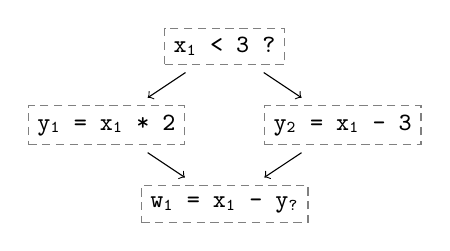
\begin{tikzpicture}[
        auto,
        block/.style={draw=black!50, thin, densely dashed, outer sep=1mm, font=\small\ttfamily},
        edge/.style={above, font=\scriptsize\ttfamily}
      ]
        \node (b1) at (0, 0)    [block] { x\textsubscript{1} < 3 ? };
        \node (b2) at (-1.5, -1)  [block] { y\textsubscript{1} = x\textsubscript{1} * 2 };
        \node (b3) at (1.5, -1)   [block] { y\textsubscript{2} = x\textsubscript{1} - 3 };
        \node (b4) at (0, -2)   [block] { w\textsubscript{1} = x\textsubscript{1} - y\textsubscript{?} };

        \draw [->] (b1) -- (b2);
        \draw [->] (b2) -- (b4);
        \draw [->] (b1) -- (b3);
        \draw [->] (b3) -- (b4);
      \end{tikzpicture}
    \end{column}

    \begin{column}{0.5\textwidth}
      \onslide<2->{%
        We introduce a Φ (phi) function to "choose" beteween
        \texttt{y\textsubscript{1}} and \texttt{y\textsubscript{2}}: \\[1.5em]

        \begin{tikzpicture}[
          auto,
          block/.style={draw=black!50, thin, densely dashed, outer sep=1mm, font=\small\ttfamily},
          edge/.style={above, font=\scriptsize\ttfamily}
        ]
          \node (b1) at (0, 0)      [block] { x\textsubscript{1} < 3 ? };
          \node (b2) at (-1.5, -1)  [block] { y\textsubscript{1} = x\textsubscript{1} * 2 };
          \node (b3) at (1.5, -1)   [block] { y\textsubscript{2} = x\textsubscript{1} - 3 };

          \node (b4) at (0, -2.5)   [block, align=left] {%
            y\textsubscript{3} = Φ(y\textsubscript{1}, y\textsubscript{2}) \\
            w\textsubscript{1} = x\textsubscript{1} - y\textsubscript{?}
          };

          \draw [->] (b1) -- (b2);
          \draw [->] (b2) -- (b4);
          \draw [->] (b1) -- (b3);
          \draw [->] (b3) -- (b4);
        \end{tikzpicture}
      }

      \vspace*{1em}
      Following the \texttt{if} block, we can simply use
      \texttt{y\textsubscript{3}}
    \end{column}
  \end{columns}
\end{frame}
  
% ---------------------------
\begin{frame}[fragile]{\currenttitle}
  SSA is useful in a number of optimizations:

  \begin{itemize}
    \item Computing constant expressions at compile-time
    \item Eliminating dead/unreachable code
    \item Replacing equivalent duplicate computations (value numbering)
    \item Etc. etc.
  \end{itemize}
\end{frame}

% ---------------------------
\renewcommand{\currenttitle}{Memory management}
\begin{frame}[fragile]{\currenttitle}
  \begin{columns}
    \begin{column}{0.6\textwidth}
      At runtime, the program must allocate memory to store data and perform
      computations:
      \begin{itemize}
        \item Statically-allocated \textbf{stack}
        \item Dynamically-allocated \textbf{heap}
        \item Read/writable static globals
        \item Literal values and constants
        \item Executable code
      \end{itemize}
    \end{column}

    \begin{column}{0.3\textwidth}
      \newcommand{\sectionn}[6]{%
        \node (#2) [
          section,
          below=0 of #3,
          minimum height=#4,
          preaction={fill, #5},
          #6
        ] {#1};%
      }
      \newcommand{\datasectionn}[3]{%
        \sectionn{#1}{#2}{#3}{5.7mm}{black!20}{font=\footnotesize}
        \draw [--, draw=black!50] (#2.north west) -- (#2.north east);%
      }

      \begin{tikzpicture}[section/.style={minimum width=3cm}]
        \node (container) [draw, minimum width=3cm, minimum height=50mm] {};

        \sectionn{Stack}{stack}{container.north}{8mm}{red!30}{}
        \draw [--, dashed, draw=black!50] (stack.south west) -- (stack.south east);

        \sectionn{Free space}{free}{stack}{12mm}{black!5}{}

        \sectionn{Heap}{heap}{free}{12mm}{yellow!30}{}
        \draw [--, dashed, draw=black!50] (heap.north west) -- (heap.north east);

        \foreach \n in {1,...,5}{
          \draw [->, draw=black!80] ($(stack.south west)+(\n{}*5mm, 1.5mm)$)  -- ($(stack.south west)+(\n{}*5mm, -2mm)$);
          \draw [->, draw=black!80] ($(heap.north west)+(\n{}*5mm, -2mm)$)    -- ($(heap.north west)+(\n{}*5mm, 1.5mm)$);
        }

        \datasectionn{Static globals}{static}{heap}
        \datasectionn{Constants}{consts}{static}
        \datasectionn{Code}{code}{consts}
      \end{tikzpicture}
    \end{column}
  \end{columns}
\end{frame}

% ---------------------------
\renewcommand{\currenttitle}{Stack management}
\begin{frame}[fragile]{\currenttitle}
  As the compiler generates lower-level code in the intermediate and back-end
  phases, it must insert code to manage function calls and stack frames:
  
  \begin{itemize}
    \item<2-> When a function is entered, a new \textbf{stack frame} is pushed to
      the stack
    \item<3-> Generated code must maintain links to upper-scope variables and
      dynamically-called function pointers
    \item<4-> The current stack frame is popped when the function is exited, and
      any return values must be placed in their correct places
  \end{itemize}
\end{frame}

% ---------------------------
\renewcommand{\currenttitle}{Heap management}
\begin{frame}[fragile]{\currenttitle}
  More often than not, the size of some object is not known at compile-time
  (e.g. arbitrary length strings or variable-size arrays) \\[1em]

  \onslide<2->{%
    Such data is stored in the \textbf{heap}, and we store \textbf{pointers} to
    that data on the stack \\[2em]
  }

  \onslide<3->{%
    The compiler must therefore insert heap allocation/freeing logic where
    appropriate
  }
\end{frame}

% ---------------------------
\begin{frame}[fragile]{\currenttitle}
  We can also use \textbf{garbage collection} \textendash{} the runtime
  monitors when heap data is no longer in use and frees it

  \only<+->
  \begin{itemize}
    \item<+-> Makes your program generally memory-safe (no access-after-free or
      double-frees)
    \item<+-> Non-trivial overhead cost; reduced execution speed
    \item<+-> Non-deterministic; program execution may experience sudden pauses
      \begin{itemize}
        \item Absolute non-starter in high-performance environments
      \end{itemize}
    \item<+-> Overzealous cleanup may destroy data still in use
  \end{itemize}
\end{frame}

% ---------------------------
\renewcommand{\currenttitle}{Back-end output}
\begin{frame}[fragile]{\currenttitle}
  As mentioned before, a compiler back-end might output different code
  depending on the target machine

  \begin{itemize}
    \item Many compilers produce assembly code for the target machine and pass
      it to an existing assembler
  \end{itemize}
\end{frame}


% ---------------------------
\renewcommand{\currenttitle}{Resource allocation}
\begin{frame}[fragile]{\currenttitle}
  The code generator must make optimal use of limited system resources: \\[2em]

  \begin{figure}
    \centering
    \begin{tikzpicture}[font=\footnotesize]
      \node (registers) [draw, minimum width=2cm]                       {Registers};
      \node (l1)        [draw, below=0 of registers, minimum width=3cm] {L1 cache};
      \node (l2)        [draw, below=0 of l1, minimum width=4cm]        {L2 cache};
      \node (main)      [draw, below=0 of l2, minimum width=5cm]        {Main memory};
      \node (disk)      [draw, below=0 of main, minimum width=6cm]      {Hard disk};

      \node (registers_t) [right=of registers]  {256KB - 8KB, 0.25 - 1ns};
      \node (l1_t)        [right=of l1]         {16KB - 64KB, 1 - 5ns};
      \node (l2_t)        [right=of l2]         {1MB - 4MB, 5 - 25ns};
      \node (main_t)      [right=of main]       {4GB - 256GB, 25 - 100ns};
      \node (disk_t)      [right=of disk]       {HUGE, 3 - 10ms};
    \end{tikzpicture}
    \caption{Memory hierarchy}
  \end{figure}
\end{frame}

% ---------------------------
\renewcommand{\currenttitle}{Register allocation}
\begin{frame}[fragile]{\currenttitle}
  In the case of native machine code, the back-end code generator must produce
  code that makes use of the CPU \textbf{registers}:

  \only<+->{}
  \begin{itemize}
    \item<+-> CPUs have a small amount of registers that they can accesss very
      quickly; computations are very fast with data inside registers
    \item<+-> A good compiler will optimize a program's use of the registers
    \item<+-> There are, of course, a couple different algorithms for allocation
  \end{itemize}
\end{frame}

% -----------------------------------------------

\end{document}
